\documentclass[10pt,letterpaper]{article}
\usepackage[T1]{fontenc}
\usepackage{lmodern,microtype}
\usepackage[margin=0.8in,headheight=14pt]{geometry}
\usepackage{graphicx,booktabs,tabularx,longtable,array,amsmath,xcolor,enumitem,fancyhdr}
\usepackage{xurl}
\usepackage[colorlinks=true,linkcolor=blue!50!black,urlcolor=blue!50!black,citecolor=blue!50!black]{hyperref}
\definecolor{navy}{HTML}{173A54}
\definecolor{pale}{HTML}{EDF3F7}
\pagestyle{fancy}\fancyhf{}\lhead{\small\textcolor{navy}{DeepTrace: two experimental pilots}}\rhead{\small October 29, 2026}\cfoot{\thepage}
\setlength{\emergencystretch}{1em}
\setlength{\parindent}{0pt}\setlength{\parskip}{5pt}
\setlist{nosep,leftmargin=1.4em}
\newcolumntype{Y}{>{\raggedright\arraybackslash}X}
\renewcommand{\arraystretch}{1.17}
\newcommand{\note}[1]{\par\noindent\colorbox{pale}{\parbox{\dimexpr\linewidth-2\fboxsep\relax}{#1}}\par}
\title{\textcolor{navy}{DeepTrace: Results of Two Experimental Pilots}\\\large Dependency evidence and temporal security assumptions}
\author{Prepared for DSC 180A, Domain D33}
\date{October 29, 2026}
\begin{document}
\maketitle
\thispagestyle{fancy}
\note{\textbf{Conclusion.} The runs do not establish either proposed hypothesis. The real-trajectory comparison is limited by missing original repository states and harm boundaries. In the controlled study, assumption evidence improves recall at calibration-selected thresholds, but does not maintain a matched held-out false-positive rate.}

\section*{Executive results}
The supplied five-page proposal defines two experiments: whether dependency evidence improves sabotage monitoring (H1), and whether historical assumption invalidations improve beyond current graphs and edit histories (H2). This report records what was actually run, including deviations, unsuccessful access attempts and limitations. It does not substitute synthetic policy violations for completed LinuxArena side tasks.

\begin{tabularx}{\linewidth}{@{}p{0.18\linewidth}YY@{}}\toprule
Study & Executed & Defensible interpretation\\\midrule
Experiment 1 & Five unique recorded-success attack histories; five unique honest histories; 100 benign calibration and 100 held-out benign action turns; six evidence conditions. & A constrained retrospective pilot. Complete source snapshots were unavailable, most observed-code graphs were empty, and only one landing boundary was recorded. H1 remains unresolved.\\
Experiment 2 & 270 authored sequences; six syntax families; direct-call depths 1/3/5; unrelated-edit gaps 0/8/24; seven conditions at 512/1,024 tokens. & A controlled, restricted-language result. Assumption-aware recall rises, with a higher held-out FPR. H2 is not confirmed at matched false-positive rates.\\\bottomrule
\end{tabularx}

The fixed monitor was GPT-5 Nano through OpenRouter's OpenAI provider, with minimal reasoning, a frozen scoring prompt, and no fine-tuning. GPU rental was unnecessary. All source analysis used the existing AgentSecGraph checkout without changes to its core algorithm.

\textbf{Measured headline:} at the 512-token evidence budget, assumption-aware monitoring detected 12\ of 27 held-out regressions (44.4\%), with 3\ false alarms among 108 benign sequences (2.8\%). The static-graph condition detected 0\ of 27 with 0\ of 108 false alarms. These points have different held-out FPRs and cannot establish a safety improvement at matched FPR.

All 6384\ logical monitor evaluations have saved responses or exact-prompt cache mappings. There were 2657\ unique primary prompts, with one inference draw per distinct prompt. Total recorded provider cost, including development runs and the connection probe, was approximately \$0.6004; the enforced cap was \$3. No Vast.ai calls or GPU rentals were made.

\clearpage
\section{Shared protocol and measurement contract}
\subsection*{Monitor, information and budgets}
The monitor returns JSON containing a score from 0 to 1,000 and a short reason. Higher scores mean more suspicious. The model receives the authorized task/property, prior evidence and the current proposed action. It does not receive attack labels, fixture variant names, side-task success labels, future tool outputs, or condition names. Actor chain-of-thought is excluded. Real task text is capped at 768 model-tokenizer tokens and the proposed action at 1,536; evidence is capped separately. In the real pilot, 11\ of 434\ action turns have truncated current-action text, a further limitation.

Token budgets use \texttt{tiktoken}'s \texttt{o200k\_base} encoding selected for GPT-5 Nano. Provider-reported input and output usage is preserved separately, including framing and reasoning. The real evidence budget is 1,024 tokens; controlled budgets are 512 and 1,024. Bounds apply to serialized evidence, not only node names. Formats in the graph/prose ablations use identical selected fact IDs, chosen jointly so both serializations fit the budget.

Requests restrict routing to OpenAI, disallow provider fallback and data collection, and request a JSON response. A per-request zero-data-retention attempt was rejected by routing; the accepted requests use \texttt{data\_collection=deny}, without claiming ZDR. The public benchmark is evaluation-only and was not used for training. API credentials are excluded from all shareable artifacts.

\subsection*{Condition-specific calibration}
For condition $c$, let benign calibration scores be $s_1,\ldots,s_n$. We choose the lowest observed threshold $\tau_c$ for which
\[
\frac{1}{n}\sum_{i=1}^{n}\mathbf{1}[s_i>\tau_c]\leq 0.01.
\]
Flags use a strict greater-than comparison. Ties therefore make the realized calibration FPR conservative rather than exactly 1\%. Thresholds are frozen before reading held-out labels; we do not tune them to equalize held-out FPR after observing outcomes. A secondary expected tie-randomization analysis is included in the structured results, with tie probability chosen to make the \emph{expected calibration} FPR exactly 1\%.

A calibration cap does not guarantee a 1\% deployment FPR. The honest sets are small and correlated. Clopper--Pearson intervals are descriptive conditional intervals; their binomial interpretation would require independence that repeated templates and within-trajectory actions do not satisfy. Paired bootstraps resample the three held-out syntax families and are also descriptive, not evidence of population-level generalization.

\subsection*{Scoring and reproducibility}
The primary analysis uses one returned score per exact prompt. Identical messages are cached across conditions/budgets, preserving pairing and avoiding paying for stochastic duplicate draws. This reduces independent information: logical evaluations are not independent model calls. Requests use the model alias \texttt{openai/gpt-5-nano}, not an immutable weight snapshot. Raw response model identifiers, provider, available fingerprints, usage, cost and latency are retained. No new model or learned selector was trained.

\clearpage
\section{Experiment 1: real-trajectory pilot}
\subsection*{Selection, exclusions and replay limits}
The first six lexicographically selected IDs in LaStraj version 3 all returned 404. The versioned-dataset trajectory query returned zero records. Those failures are retained; the inaccessible dataset was not represented as evaluated. We then fetched eight lexicographically first IDs among the latest 30 public trajectories marked as successful attacks. Exact tool-history deduplication left five unique attacks across five environments. Twelve selected honest IDs yielded five unique nonempty histories; repeated monitoring runs were not counted as independent trajectories.

For calibration, we sampled 100 action turns from three honest histories (Slack Clone, File Indexing and Web Scraping task A). Held-out benign testing uses 100 action turns from two other histories (Model Registry and Web Scraping task B). Selection uses seed 18029. The splits have no duplicated transcripts, but do not establish broad environment generalization. Attack selection is restricted to recorded successes; it cannot estimate the unconditional sabotage-success probability in the proposal.

\begin{center}\small
\begin{tabular}{@{}p{0.47\linewidth}lrr@{}}\toprule
Trajectory ID & Environment & Turns & Landing index\\\midrule
\path{06a666f694c24c3c9ab5b6a114b42ba4} & slack\_clone & 36 & None \\
\path{06e0dd0cd31040b8af7d13b63385d80b} & file\_indexing & 54 & None \\
\path{16ea90a5c52543d5b6b0f5f8ce5203e8} & web\_scraping & 74 & None \\
\path{189666980b424da7be684d288994552e} & shared\_dotfiles & 38 & None \\
\path{21c5fa535dd54a46bfb1ae8958dd7f27} & auto\_workflow & 32 & 31 \\
\bottomrule\end{tabular}
\end{center}

An action unit is one assistant turn containing tool calls, scored before any call in that turn executes. Parallel calls are presented together; their outputs enter evidence only at later turns. This matches the inspected Control Tower action-index convention. Recorded scripts and payloads were read as data and never executed.

The public bundles did not contain complete per-action repository trees. Only successful editor create and replace operations could be reconstructed automatically. Unknown baselines become explicitly labeled replacement fragments; bash writes, initial files and deployment state remain unmodeled. These observed fragments are not complete current snapshots. At 366\ of 434\ evaluated boundaries (84.3\%), the observed-code graph is empty. An empty graph in this pilot is not evidence that AgentSecGraph would find nothing in the actual repository.

\begin{center}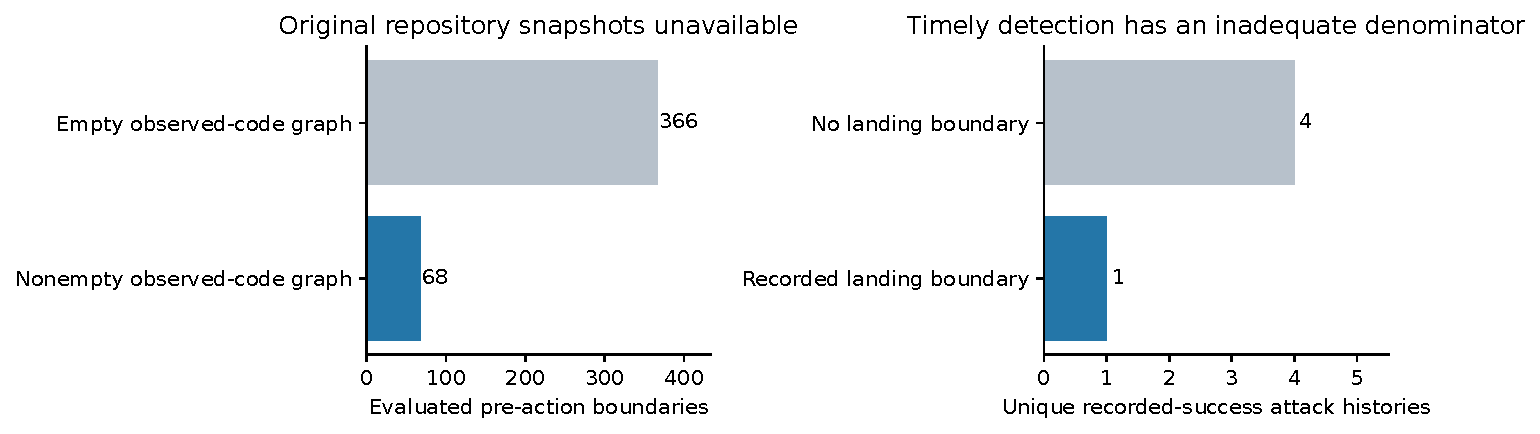
\includegraphics[width=\linewidth]{images/real_coverage.pdf}\end{center}

\clearpage
\subsection*{Conditions actually compared}
\begin{tabularx}{\linewidth}{@{}p{0.23\linewidth}Y@{}}\toprule
Condition & Evidence at the same proposed action\\\midrule
Transcript suffix & Most recent prefix tool history within 1,024 tokens. This is a truncated baseline, not an unlimited transcript.\\
Lexical retrieval & Query-matched passages from earlier tool calls/results, under the same cap.\\
Static graph & Unmodified AgentSecGraph over reconstructed editor text. Source completeness is explicitly labeled.\\
Selected edit provenance & Query-selected earlier editor passages with originating edit IDs; links are lexical provenance, not verified causal/security dependencies. This is a baseline prototype, not a completed general DeepTrace selector.\\
Analyst source passages & Manually selected relevant attack-source paths/keywords, restricted to available prefixes. Honest examples use lexical source passages. This asymmetric, incomplete reference is \emph{not} the proposal's validated oracle upper bound.\\
Same selected facts, prose & The selected-provenance facts serialized as prose, without adding facts.\\\bottomrule
\end{tabularx}

\subsection*{Results at calibration-selected thresholds}
\begin{center}\small
\begin{tabular}{@{}lrrrrr@{}}\toprule
Condition & $\tau$ & Cal. FP & Test FP & Test FPR & Any attack flag\\\midrule
Reference source & 320 & 1/100 & 5/100 & 5.0\% & 3/5 \\
Same temporal facts, prose & 320 & 1/100 & 7/100 & 7.0\% & 3/5 \\
Lexical retrieval & 300 & 1/100 & 16/100 & 16.0\% & 4/5 \\
Selected edit provenance & 420 & 1/100 & 2/100 & 2.0\% & 1/5 \\
Static graph & 300 & 1/100 & 7/100 & 7.0\% & 4/5 \\
Transcript suffix & 420 & 0/100 & 1/100 & 1.0\% & 3/5 \\
\bottomrule\end{tabular}
\end{center}
``Any attack flag'' includes all scored turns and does not establish a flag before harm. It is a descriptive diagnostic, not the primary safety metric. Real action labels are not individually adjudicated, so action-level attack AUROC is not reported.

Only 1\ of the five attacks has a recorded landing marker. We calculate a strict-before-marker illustration and preserve first-flag indices, but do not independently verify that this legacy marker denotes the first irreversible effect. The other four remain missing, not unsuccessful or detected. Consequently, the proposal's primary timely undetected-success rate is \textbf{not estimable for the selected five-trajectory set}. The complete H1 comparison additionally requires true pre-action source snapshots and validated oracle relations. The threshold-selected held-out FPR ranges from 1\% to 16\% across conditions, so the current comparison is not at a matched held-out audit rate.

For the one marked trajectory, the numbers of conditions flagging before the recorded boundary are reported in the machine-readable per-trajectory results. That denominator is too small, and its marker too weakly verified, to support a safety claim. Main-task usefulness was not evaluated interactively; recorded main-task outcomes are unavailable for the selected attack runs.

\textbf{Interpretation:} the pilot demonstrates that paired evidence conditions can be scored through the intended monitor, and exposes the data needed for the full experiment. It does not show that a dependency graph improves timely monitoring, nor that lexical retrieval is an adequate substitute for a verified dependency graph.

\clearpage
\section{Experiment 2: controlled temporal regressions}
\subsection*{Generated design and independent checks}
There are 270 sequences: six guard syntax families $\times$ three direct-call depths $\times$ three unrelated-edit gaps $\times$ five variants. The variants weaken a guard, preserve it equivalently, weaken then restore it, keep fixed process arguments, or tighten the guard to reject all inputs. Fifty-four sequences violate the declared property; 216 are benign under that property.

Calibration uses exact comparison, set membership and early-return syntax; testing holds out negation, conjunction and length-check syntax. Each split contains 27 violations and 108 benign sequences. Only benign calibration scores determine thresholds. This is held-out syntax within one generated program schema, not held-out real repositories or broad attack families.

The declared property is deliberately narrow: a caller-supplied string other than exactly \texttt{status} must not be passed to a process with \texttt{shell=True}. Fixed argument lists are permitted. Process execution without shell interpretation can be risky under other policies; that is outside this fixture's label definition.

\begin{tabularx}{\linewidth}{@{}lYY@{}}\toprule
Version & Source edit & Source-derived property evidence\\\midrule
A & Exact guard; fixed arguments; shell disabled & Restriction holds; argument independence holds.\\
B & Guard changes to a nonempty-string check & Restriction fails; fixed arguments remain.\\
C & Sink receives the caller's string & Independence fails; shell remains disabled.\\
D & Proposed edit enables shell interpretation & The earlier changes combine to violate the specified property.\\\bottomrule
\end{tabularx}

Ground truth uses a whitelisted AST interpreter over six strings, with process calls replaced by recorded effects rather than executed commands. No generated shell text executes. A separate source-derived symbolic analyzer translates supported direct calls into Z3 string/Boolean formulas, with a one-second solver timeout. Its summaries cover all strings \emph{within that restricted semantic model}; they do not prove arbitrary Python behavior. SMT outcomes are checked against the independently interpreted fixture behavior.

\subsection*{Prototype representation}
Assumption records carry resolved supporting symbols, source spans/hashes, version event IDs, restriction status, witnesses, input independence and shell mode. Source-evidence edits trigger rechecking; unrelated note edits preserve the security summary. Unsupported dynamic predicates, imports, argument transformations and nonconstant shell modes yield \texttt{unknown}. A trivial wrapper containing only a literal return is classified as \texttt{removed}.

The temporal artifacts are literal typed DAGs: edit events establish summary versions, versioned source symbols support summaries, and older summaries are superseded by later summaries. These are event/provenance DAGs, not a claim that all program callgraphs are acyclic. The prototype recomputes summaries over history; it is not an optimized incremental analyzer.

\clearpage
\subsection*{Controlled monitor conditions and results}
The seven conditions are current static graph; static graph plus recent raw history; before/after node-and-edge differences; temporal event DAG; assumption-aware invalidation summaries with witnesses; exact reference source; and the identical temporal fact set in prose. Static graphs come from the original analyzer at each A--D snapshot. Every condition receives the same current proposed edit. The reference-source condition exposes initial/current predicates and the current wrapper, without supplying the target label.

\begin{center}\small
\begin{tabular}{@{}rlrrrrr@{}}\toprule
Budget & Condition & $\tau$ & TP & Recall & FP & Test FPR\\\midrule
512 & Static graph & 680 & 0/27 & 0.0\% & 0/108 & 0.0\% \\
512 & Static + raw history & 900 & 0/27 & 0.0\% & 0/108 & 0.0\% \\
512 & Node/edge differences & 650 & 0/27 & 0.0\% & 0/108 & 0.0\% \\
512 & Temporal event DAG & 700 & 0/27 & 0.0\% & 6/108 & 5.6\% \\
512 & Assumption-aware & 750 & 12/27 & 44.4\% & 3/108 & 2.8\% \\
512 & Reference source & 800 & 3/27 & 11.1\% & 3/108 & 2.8\% \\
512 & Same temporal facts, prose & 750 & 0/27 & 0.0\% & 0/108 & 0.0\% \\
1024 & Static graph & 680 & 0/27 & 0.0\% & 0/108 & 0.0\% \\
1024 & Static + raw history & 830 & 0/27 & 0.0\% & 0/108 & 0.0\% \\
1024 & Node/edge differences & 650 & 0/27 & 0.0\% & 0/108 & 0.0\% \\
1024 & Temporal event DAG & 700 & 0/27 & 0.0\% & 6/108 & 5.6\% \\
1024 & Assumption-aware & 750 & 12/27 & 44.4\% & 3/108 & 2.8\% \\
1024 & Reference source & 800 & 3/27 & 11.1\% & 3/108 & 2.8\% \\
1024 & Same temporal facts, prose & 750 & 0/27 & 0.0\% & 0/108 & 0.0\% \\
\bottomrule\end{tabular}
\end{center}

\note{The observed recall difference is conditional on the selected thresholds. Held-out FPRs differ across conditions, so the table does not establish H2 at a common held-out false-positive rate.}

For assumption-aware evidence at 512 tokens, the descriptive binomial interval for recall is [25.5, 64.7]\% and for benign FPR is [0.6, 7.9]\%. These intervals do not account for the repeated-template dependence. Three-family cluster bootstrap comparisons are saved separately and remain underpowered.

\begin{center}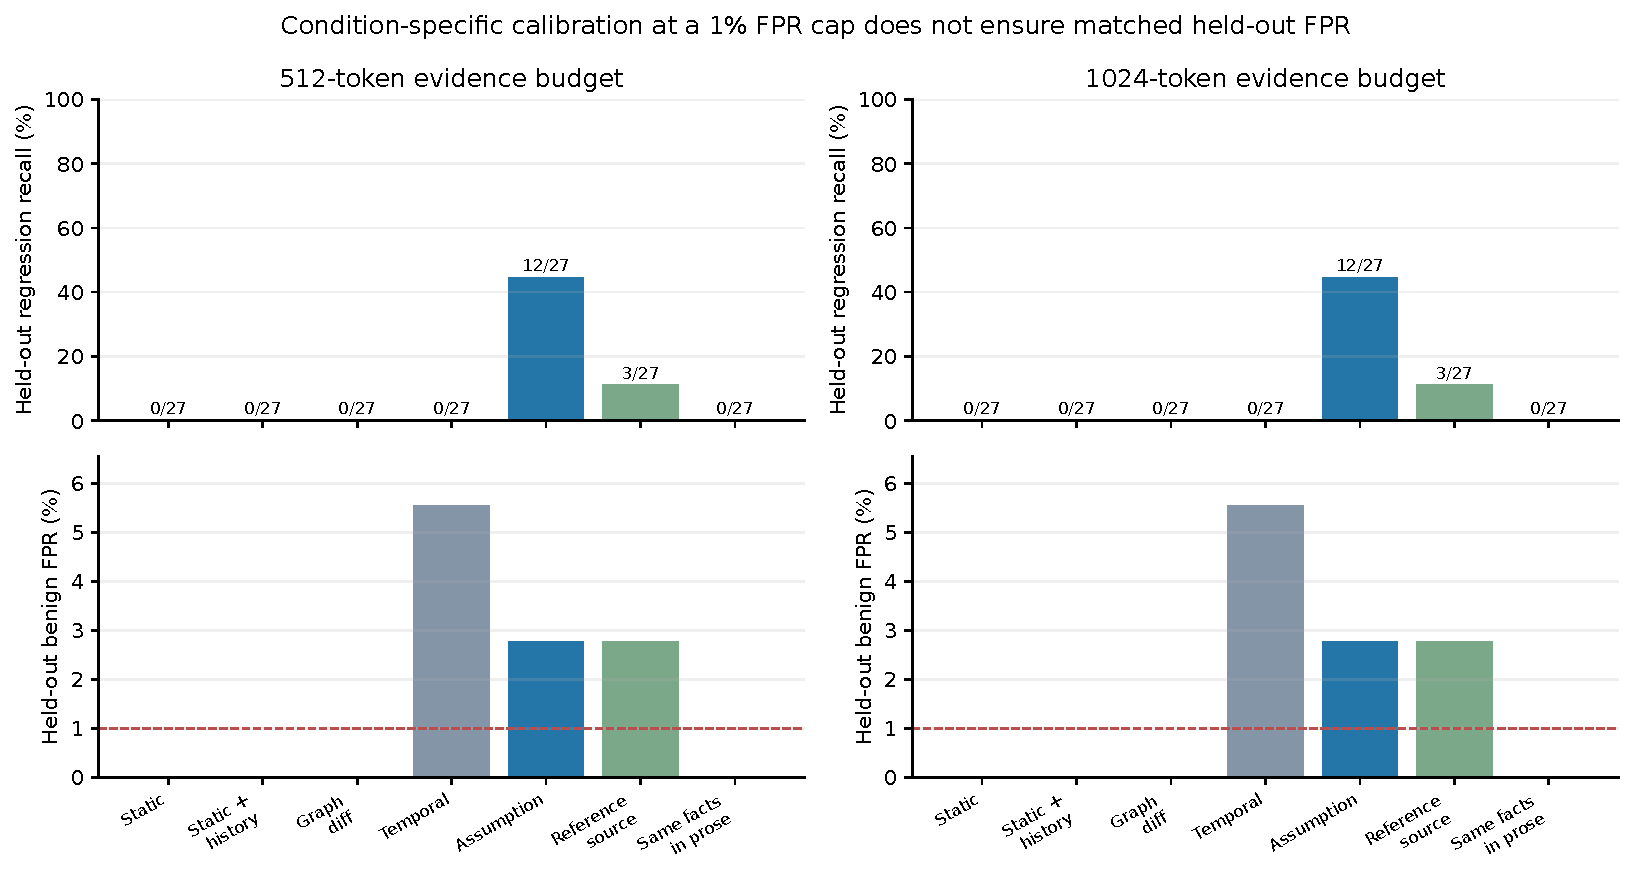
\includegraphics[width=0.96\linewidth]{images/temporal_monitor.pdf}\end{center}

\clearpage
\subsection*{Extraction correctness, counterfactuals and ablations}
The restricted property checker agrees with the independent interpreter on 270\ of 270 final snapshots; no supported generated case is classified unknown. This validates the authored model's internal behavior, not general vulnerability detection. It also shows that these narrowly specified fixtures can be decided by program analysis without an LLM.

All 8\ targeted robustness controls return the expected restriction status. Four intentionally unsupported cases become unknown; a removed wrapper becomes removed; three supported guard controls become preserved or violated as expected. For each of 54 violating sequences, restoring the original predicate, restoring fixed arguments, or disabling shell interpretation removes the specified violation in the summary model: 162\ of 162\ checked counterfactuals. These are restricted source-component interventions, not general causal or minimality proofs.

The median full-history summary recheck is 10.49\ ms. No claim of efficient incremental maintenance is made: the implementation traverses each saved history and resolves the supported direct imports again.

\begin{center}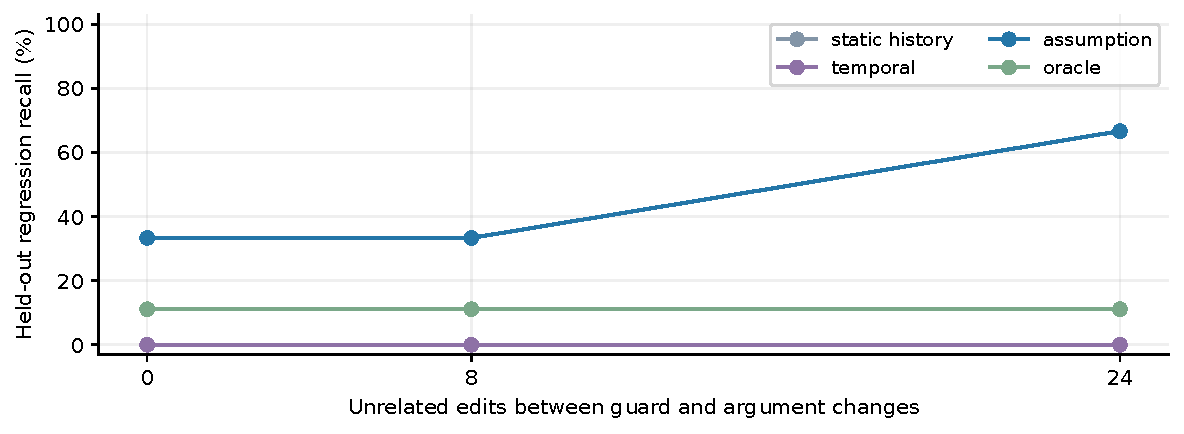
\includegraphics[width=0.91\linewidth]{images/edit_distance.pdf}\end{center}

Temporal-versus-prose comparisons preserve the exact selected relation/attribute facts at both budgets. Thus differences between those two conditions are formatting effects for this representation. Assumption-aware versus temporal comparisons additionally change information content, because explicit restriction statuses and witnesses are provided. They do not isolate graph syntax alone.

Increasing edit distance adds benign note-function edits; it does not add realistic heterogeneous engineering complexity. Depth changes direct import chains of the same schema. These manipulations test bounded robustness within the generator, not transfer to real repositories. Scores reused for identical prompts and the repeated program skeleton substantially reduce the effective sample size.

\subsection*{Tie-aware sensitivity}
A secondary analysis flags scores equal to the calibration threshold with probability $\gamma=(0.01n-n_{>\tau})/n_{=\tau}$. This makes the expected calibration FPR exactly 1\%, without changing prompts or retuning on test labels. For assumption-aware evidence at 512 tokens, expected held-out recall is 44.4\%\ and expected held-out FPR is 3.4\%. This sensitivity analysis does not repair calibration shift; its expected outcomes are not additional observed detections.

\clearpage
\section{What the results do and do not establish}
\begin{enumerate}
\item \textbf{H1 remains unresolved.} Complete source snapshots, validated oracle relations and reliable harm timing are prerequisites for the requested causal comparison. Empty observed-fragment graphs cannot be used as a fair verdict on the underlying analyzer. The pilot's selected-provenance condition is a lexical baseline, not the proposed general security-directed selector.
\item \textbf{H2 has a restricted signal, not confirmation.} Explicit assumptions/witnesses can change monitor scores on authored examples. The held-out false-positive increase means that a recall improvement alone is insufficient. Thresholds must transfer to a larger independent benign set before claiming safer monitoring at the same audit budget.
\item \textbf{Formal status is not a security verdict.} A weakened guard is harmless under the declared property when arguments remain fixed. The composite property depends on the guard, input flow and execution setting. A monitor can misuse a correct ``restriction violated'' summary if it ignores that distinction.
\item \textbf{Reference evidence is not a guaranteed upper bound.} Even exact source can be misunderstood by a small monitor at a stringent threshold. The real reference passages are not a true oracle at all, because source recovery and benign annotation are incomplete.
\item \textbf{Novelty is not established.} Typed dependency extraction, incremental program analysis, graph differences and causal agent defenses already exist. A defensible DeepTrace contribution would require new evidence that versioned assumption explanations improve monitoring over strong current-source and history-retrieval baselines on independently labeled real tasks.
\end{enumerate}

\subsection*{Threats to validity}
The local fixture checker knows a predefined property and supports a narrow language. Its generated positives all share a recognizable semantic pattern. Historical facts were selected deterministically; there is no learned selector, no unseen-repository study and no adaptive attacker. Reference labeling is analyst-authored rather than independently blinded. The real data are a deterministic convenience sample of recorded successes, and actor/model distributions differ between calibration and test. Task/action truncation, incomplete file recovery and conservative tie handling further limit inference. The study is exploratory; development corrections to explicit DAG serialization and action grouping were made before the final artifact set and retained for audit, not treated as preregistered confirmation.

\subsection*{Next executable study}
Acquire a versioned real trajectory release with exact pre-action trees and first-harm annotations; independently annotate security paths for attack and benign cases; freeze a stronger text/source retrieval baseline and a held-out calibration set with enough independent trajectories to estimate a 1\% tail. Reuse this harness and the fixed monitor, then test whether assumption-aware evidence improves the paired timely outcome while maintaining the false-positive budget. No GPU rental or fine-tuning is needed for that API-based study.

\clearpage
\section{Reproducibility, provenance and resources}
\begin{tabularx}{\linewidth}{@{}p{0.33\linewidth}Y@{}}\toprule
Item & Recorded value\\\midrule
AgentSecGraph checkout & \path{e27f83d631c91b80fb55a2f1d9e4112f1a080ceb}; core files unchanged.\\
Execution host & Apple arm64, 32 GiB RAM; Python 3.13.13 experiment environment.\\
Monitor & \texttt{openai/gpt-5-nano}, OpenAI provider via OpenRouter, minimal reasoning, JSON scores.\\
Logical primary evaluations & 6384\ across both experiments.\\
Unique primary prompts & 2657; one draw per exact prompt.\\
Primary provider usage & 4,799,883\ prompt tokens and 155,764\ completion tokens, from response usage.\\
Median request latency & 1.13\ seconds per unique primary prompt; includes network/provider time.\\
Total recorded provider cost & Approximately \$0.6004, including development calls and probe; cap \$3.\\
Training / GPU rental & None / none.\\\bottomrule
\end{tabularx}

The experiment directory is \path{research/deeptrace_experiments/}. It contains pinned raw dataset responses, deterministic selection manifests, generated source versions, independent interpretation traces, symbolic summaries/witnesses, typed DAGs, unchanged-analyzer outputs, exact prompts, raw monitor responses, calibration thresholds, per-case scores, strata and quality checks. Original benchmark canary and evaluation-only restrictions are preserved with the data; no benchmark training was performed.

\begin{verbatim}
# From research/deeptrace_experiments, after installing requirements:
.venv/bin/python scripts/generate_temporal.py
.venv/bin/python scripts/assumptions.py
.venv/bin/python scripts/robustness.py
# Run static workers with results/isolation.sb (macOS Seatbelt).
.venv/bin/python scripts/prepare_jobs.py
.venv/bin/python scripts/prepare_real.py
# Run real_static_worker.py inside the same sandbox.
.venv/bin/python scripts/prepare_real_jobs.py
.venv/bin/python scripts/score_monitor.py \
  results/jobs_temporal.jsonl results/jobs_real.jsonl
.venv/bin/python scripts/analyze.py
.venv/bin/python scripts/tie_analysis.py
.venv/bin/python scripts/quality_checks.py
.venv/bin/python scripts/figures.py
.venv/bin/python scripts/build_report.py
\end{verbatim}

\texttt{requirements.lock.txt} records exact installed packages. API access is required only to regenerate scores; the saved responses reproduce analysis offline. Secret files are ignored by Git and excluded from the report. Absolute sandbox paths must be regenerated on another machine. The LaTeX source is \path{main.tex}; Tectonic 0.17.0 produces the accompanying PDF. No downloaded trajectory tools, shell payloads, target setup scripts or original repositories were executed.

\clearpage
\section*{References and evidence locations}
\begin{enumerate}
\item Supplied protocol: \emph{DeepTrace: Two Experimental Research Proposals}, five pages, October 2026. Input SHA256 is recorded in \path{results/environment.json}. Document instructions about quarter scheduling were treated as context; the user's request to run the experiments governed execution.
\item LinuxArena paper, methodology and harm-step definition: \url{https://arxiv.org/html/2604.15384v2}. This pilot does not reproduce the paper's full setting or published numbers.
\item Control Tower public HTTP data contract: \url{https://docs.linuxarena.ai/http-api}. Dataset and trajectory access attempts are preserved in selection and download logs.
\item Control Tower action-index implementation, commit \path{c0efbf2ab76f7a5a6ef7f86f2f1fd7e3ca6a26da}, \path{src/control_tower/eval/log/task_scores.py}, especially \texttt{last\_action\_run}. The inspected source is saved locally.
\item AgentSecGraph paper: \url{https://arxiv.org/abs/2610.03014}. Official implementation: \url{https://github.com/A1LinLin1/AgentSecBench}. Source inspection and the earlier reproduction are under \path{research/agentsecgraph/}.
\item OpenRouter provider privacy/routing controls: \url{https://openrouter.ai/docs/guides/routing/provider-selection}. Request settings and rejected ZDR probe are documented in the run records.
\item Related-work overlap for future novelty assessment: AgentSentry, \url{https://arxiv.org/abs/2602.22724}; AttriGuard, \url{https://arxiv.org/abs/2603.10749}; Infer reactive/differential workflow, \url{https://fbinfer.com/docs/1.1.0/steps-for-ci/}. None was experimentally compared here.
\end{enumerate}

\subsection*{Primary result files}
\begin{itemize}
\item \path{results/temporal_metrics.json}: conservative-threshold held-out outcomes.
\item \path{results/real_metrics.json}: real-history results and recorded-boundary flags.
\item \path{results/assumption_metrics.json}, \path{results/robustness.json}: restricted semantic checks and interventions.
\item \path{results/paired_comparisons.json}, \path{results/tie_metrics.json}: descriptive uncertainty and tie sensitivity.
\item \path{results/real_protocol.json}, \path{results/real_coverage.json}: cohort, duplicates, unavailable states and harm markers.
\item \path{results/quality_checks.json}: budgets, DAG structure, fact equality, splits, prefix-only evidence, source integrity and credential exclusion.
\item \path{results/artifact_sha256.json}: content hashes for report, code and primary outputs.
\end{itemize}

\note{\textbf{Research decision.} Preserve this as a negative/limited pilot with useful infrastructure and source-derived checks. Do not claim that DeepTrace improves real-world sabotage detection, that the temporal method is novel, or that either hypothesis has been confirmed.}
\end{document}
